\documentclass[svgnames,11pt]{beamer}
\input{/home/tof/Documents/Cozy/latex-include/preambule_commun.tex}
\input{/home/tof/Documents/Cozy/latex-include/preambule_beamer.tex}
%\usepackage{pgfpages} \setbeameroption{show notes on second screen=left}
\author[]{Christophe Viroulaud}
\title{Exercices encodage\\correction}
\date{\framebox{\textbf{DonRep 15}}}
%\logo{}
\institute{Première - NSI}

\begin{document}
\begin{frame}
    \titlepage
\end{frame}
\section{Exercice 1}
\begin{frame}
    \frametitle{Exercice 1}

    \begin{enumerate}
        \item Les caractères sont notés en hexadécimal.
        \item Attention le 20 est en hexadécimal; il s'agit donc en binaire de 0010 0000.
        \item En décimal $00100000 = 2^5 = 32$
        \item VIVE LES VACANCES
    \end{enumerate}

\end{frame}
\section{Exercice 2}
\begin{frame}
    \frametitle{Exercice 2}

    \begin{enumerate}
        \item U+0040 en binaire: 0100 0000
        \item Il suffit d'un octet pour encoder ce caractère en UTF-8.
        \item Le point de code de la lettre Ê est U+00CA. En binaire on a: 1100 1010. Il faut alors 2 octets pour encoder ce caractère en UTF-8.

              On utilise la suite d'octets: 110xxxxx 10xxxxxx et on remplace les \emph{x} par les chiffres binaires. On complète avec des 0:
              \begin{center}
                  110\textbf{00011} 10\textbf{001010}

              \end{center}
    \end{enumerate}

\end{frame}
\section{Exercice 3}
\begin{frame}
    \frametitle{Exercice 3}
    Pour convertir en binaire il faut effectuer des divisions successives par 2.
    
    \begin{center}
        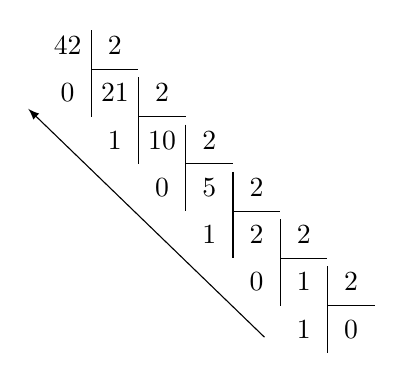
\begin{tikzpicture}
            \node at(0,0){42};
            \node at(0.6,0){2};
            \node at(0,-0.6){0};
            \node at(0.6,-0.6){21};
            \draw (0.3,0.2)--(0.3,-0.9);
            \draw (0.3,-0.3)--(0.9,-0.3);
    
            \node at(1.2,-0.6){2};
            \node at(0.6,-1.2){1};
            \node at(1.2,-1.2){10};
            \draw (0.9,-0.4)--(0.9,-1.5);
            \draw (0.9,-0.9)--(1.5,-0.9);
    
            \node at(1.8,-1.2){2};
            \node at(1.2,-1.8){0};
            \node at(1.8,-1.8){5};
            \draw (1.5,-1.0)--(1.5,-2.1);
            \draw (1.5,-1.5)--(2.1,-1.5);
    
            \node at(2.4,-1.8){2};
            \node at(1.8,-2.4){1};
            \node at(2.4,-2.4){2};
            \draw (2.1,-1.6)--(2.1,-2.7);
            \draw (2.1,-2.1)--(2.7,-2.1);
    
            \node at(3.0,-2.4){2};
            \node at(2.4,-3.0){0};
            \node at(3.0,-3.0){1};
            \draw (2.7,-2.2)--(2.7,-3.3);
            \draw (2.7,-2.7)--(3.3,-2.7);
    
            \node at(3.6,-3.0){2};
            \node at(3.0,-3.6){1};
            \node at(3.6,-3.6){0};
            \draw (3.3,-2.8)--(3.3,-3.9);
            \draw (3.3,-3.3)--(3.9,-3.3);
            \draw [->,>=latex] (2.5,-3.7) -- (-0.5,-0.8);
        \end{tikzpicture}
        \captionof{figure}{$42_{10}=101010_2$}
    \end{center}
\end{frame}
\begin{frame}[fragile]
    \frametitle{}

\begin{center}
\begin{lstlisting}[language=Python , basicstyle=\ttfamily\small, xleftmargin=2em, xrightmargin=2em]
def deci_bin(entier: int) -> str:
    res = ""
    while entier > 0:
        res = str(entier % 2)+res
        entier = entier//2
    return res
\end{lstlisting}
\end{center}    

\end{frame}
\begin{frame}
    \frametitle{}

    \begin{center}
        \begin{tabular}{|*{5}{c|}}
            \hline
            S&A&L&U&T\\
            \hline
            83& 65& 76& 85&84\\
            \hline
        \end{tabular}
    \end{center}

\end{frame}
\begin{frame}[fragile]
    \frametitle{}

\begin{center}
\begin{lstlisting}[language=Python , basicstyle=\ttfamily\small, xleftmargin=2em, xrightmargin=2em]
def decoder(code_car: list) -> str:
    res = ""
    for code in code_car:
        res = res+chr(code)
    return res
\end{lstlisting}
\end{center}
\begin{center}
\begin{lstlisting}[language=Python , basicstyle=\ttfamily\small, xleftmargin=2em, xrightmargin=2em]
print(decoder([83, 65, 76, 85, 84]))
# affiche 'SALUT'
\end{lstlisting}
\captionof{code}{Appel de la fonction}
\label{CODE}
\end{center}
\end{frame}
\section{Exercice 4}
\begin{frame}
    \frametitle{Exercice 4}

\begin{aretenir}[Documentation]
    def ord(c: Text) -> int\\
    Return the Unicode code point for a one-character string.
\end{aretenir}
\begin{aretenir}[Documentation]
    def hex(i: int) -> str\\
    Return the hexadecimal representation of an integer.
    
    hex(12648430)\\
    '0xc0ffee'
\end{aretenir}
\end{frame}
\begin{frame}[fragile]
    \frametitle{}

\begin{center}
\begin{lstlisting}[language=Python , basicstyle=\ttfamily\small, xleftmargin=2em, xrightmargin=2em]
def utf8(car: str) -> str:
    return hex(ord(car))
\end{lstlisting}
\end{center} 
\begin{center}
\begin{lstlisting}[language=Python , basicstyle=\ttfamily\small, xleftmargin=2em, xrightmargin=2em]
>>> utf8("é")
0xE9
\end{lstlisting}
\captionof{code}{Appel de la fonction}
\label{CODE}
\end{center}
\end{frame}
\begin{frame}[fragile]
    \frametitle{}

\begin{center}
\begin{lstlisting}[language=Python , basicstyle=\ttfamily\small, xleftmargin=2em, xrightmargin=2em]
def encoder_hexa(phrase: str) -> list:
    codes = []
    for lettre in phrase:
        codes.append(utf8(lettre))
    return codes
\end{lstlisting}
\end{center} 
\begin{center}
\begin{lstlisting}[language=Python , basicstyle=\ttfamily\small, xleftmargin=2em, xrightmargin=2em]
>>> encoder_hexa("éléphant")
['0xe9', '0x6c', '0xe9', '0x70', '0x68', '0x61', '0x6e', '0x74']
\end{lstlisting}
\captionof{code}{Appel de la fonction}
\label{CODE}
\end{center}   

\end{frame}
\begin{frame}[fragile]
    \frametitle{}

\begin{center}
\begin{lstlisting}[language=Python , basicstyle=\ttfamily\small, xleftmargin=2em, xrightmargin=2em]
def encoder_hexa2(phrase: str) -> list:
    # crée un tableau à la bonne dimension
    codes = ["" for _ in range(len(phrase))]
    
    for i in range(len(phrase)):
        codes[i] = utf8(phrase[i])
    return codes
\end{lstlisting}
\captionof{code}{Seconde version}
\end{center} 
\begin{center}
\begin{lstlisting}[language=Python , basicstyle=\ttfamily\small, xleftmargin=2em, xrightmargin=2em]
>>> encoder_hexa2("éléphant")
['0xe9', '0x6c', '0xe9', '0x70', '0x68', '0x61', '0x6e', '0x74']
\end{lstlisting}
\captionof{code}{Appel de la fonction}
\label{CODE}
\end{center}   

\end{frame}
\end{document}